%% AMS-LaTeX Created with the Wolfram Language : www.wolfram.com

\documentclass[12pt]{article}

\usepackage[letterpaper,margin=1in]{geometry}
\usepackage{amsmath,amssymb,setspace}
\usepackage{graphicx}
\usepackage{bm}
\graphicspath{{./figs/}}
\usepackage{tcolorbox}
\usepackage[framed,numbered,autolinebreaks,useliterate]{mcode}
\usepackage{enumitem}
\usepackage{xcolor}
\usepackage{listings}
\usepackage{hyperref}
\usepackage[cal=boondox]{mathalfa}
\usepackage{tikz} % for the neural network diagram

% Define colors for lstlisting
\definecolor{codegreen}{rgb}{0,0.6,0}
\definecolor{codegray}{rgb}{0.5,0.5,0.5}
\definecolor{codepurple}{rgb}{0.58,0,0.82}
\definecolor{backcolour}{rgb}{0.95,0.95,0.95}

\lstdefinestyle{mystyle}{
    backgroundcolor=\color{backcolour},   
    commentstyle=\color{codegreen},
    keywordstyle=\color{magenta},
    numberstyle=\tiny\color{codegray},
    stringstyle=\color{codepurple},
    basicstyle=\ttfamily\normalsize,
    breakatwhitespace=false,         
    breaklines=true,                 
    captionpos=b,                    
    keepspaces=true,                 
    numbers=none,  
    columns=flexible,         
    numbersep=5pt,                  
    showspaces=false,                
    showstringspaces=false,
    showtabs=false,                  
    tabsize=2,
    literate={'}{{\textquotesingle}}1 {''}{{\textquotedbl}}2
}
\lstset{style=mystyle}

\hypersetup{
    colorlinks=true,
    linkcolor=blue,
    filecolor=magenta,      
    urlcolor=cyan,
    pdftitle={Your Document Title},
    pdfpagemode=FullScreen,
}

\def\mathbi#1{\textbf{\em #1}}
\newcommand{\fullunderline}{\noindent\makebox[\linewidth]{\rule{\linewidth}{0.1pt}}\\[-2em]}

\begin{document}
\doublespacing	

\title{CE 401/5501 Homework 04\\[2in]
\textbf{Name: \rule{2in}{0.15mm}}}
\author{}
\date{}
\maketitle

\newcommand*{\I}{\imath} % imaginary unit i

\newpage

\section{Multiple Choice / Fill-in-the-blank Questions}

\textbf{Question 1} \\

A perceptron is the simplest artificial neural network, and its mathematical expression can be written as 
\[
y=f[u(\bm{x})],
\]
where \( u(\bm{x}) = \bm{w}^T \bm{x} + b \). Which of the following statements describe its architecture?

\begin{itemize}
    \item [$\checkmark$] The functional model describes a computing flow: Input features \(\bm{x}\) \(\rightarrow\) aggregation through \(u(\cdot)\) \(\rightarrow\) activation through \(f(\cdot)\) \(\rightarrow\) outputting a class label or score \(y\).
    \item [$\checkmark$] \(f(\cdot)\) is called an activation function, which is often a simple nonlinear function.
    \item [$\square$] The perceptron model is equivalent to a logistic regression model.
    \item [$\square$] The output \(y\) must be binary.
\end{itemize}

\vspace{1em}
\textbf{Question 2} \\

Given a perceptron model for binary classification, its input is a two-dimensional data point denoted by 
\[
\bm{x} = \begin{bmatrix} x_1 \\ x_2 \end{bmatrix}.
\]
After learning from the data, the resulting learned weights and bias are 
\[
[w_1, w_2, b]^T = [-4, -3, 10]^T.
\]
Answer the following:

\begin{enumerate}[label=(\alph*)]
    \item \textbf{Decision function:} \\
    The decision function is given by
    \[
    u(\bm{x}) = -4x_1 - 3x_2 + 10.
    \]
    
    \item \textbf{Decision boundary:} \\
    The decision boundary is defined by \( u(\bm{x})=0 \). Solving for \(x_2\) as a function of \(x_1\):
    \[
    -4x_1 - 3x_2 + 10 = 0 \quad \Longrightarrow \quad x_2 = \frac{10}{3} - \frac{4}{3}x_1.
    \]
    
    \item \textbf{Perceptron model with Heaviside activation:} \\
    When using the Heaviside step function \(H(\cdot)\), the perceptron model is:
    \[
    y = H(u(\bm{x})) = H(-4x_1 - 3x_2 + 10),
    \]
    where
    \[
    H(u) = \begin{cases} 1, & u \ge 0, \\ 0, & u < 0. \end{cases}
    \]
    
    \item \textbf{Labeling data points:} \\
    Given the data points:
    \begin{itemize}
        \item Point A: \(\bm{x}_A = \begin{bmatrix} 1 \\ 4 \end{bmatrix}\) \\
        Compute:
        \[
        u(\bm{x}_A) = -4(1) - 3(4) + 10 = -4 - 12 + 10 = -6.
        \]
        Since \(-6 < 0\), Point A is labeled as \(0\).
        
        \item Point B: \(\bm{x}_B = \begin{bmatrix} -2 \\ 2 \end{bmatrix}\) \\
        Compute:
        \[
        u(\bm{x}_B) = -4(-2) - 3(2) + 10 = 8 - 6 + 10 = 12.
        \]
        Since \(12 \ge 0\), Point B is labeled as \(1\).
    \end{itemize}
    
    \item \textbf{Predicted scores with ReLU activation:} \\
    Using the ReLU activation defined by
    \[
    \text{ReLU}(u) = \max(0,u),
    \]
    the predicted scores are:
    \begin{itemize}
        \item For Point A:
        \[
        \text{ReLU}(-6) = 0.
        \]
        \item For Point B:
        \[
        \text{ReLU}(12) = 12.
        \]
    \end{itemize}
\end{enumerate}

\vspace{1em}
\textbf{Question 3} \\

A civil engineer is constructing a machine learning exercise where each data point is a \(3\times 1\) vector and there are two class labels, 0 and 1. The engineer collected 1000 data points with manual labels. The initial neural network is configured as follows:
\begin{itemize}
    \item The network has two hidden layers. Each hidden layer contains 5 neurons.
    \item The network is fully connected (i.e., a multilayer perceptron) and includes bias (intercept) parameters at every layer. (At each layer, an additional constant input of 1 is used.)
\end{itemize}
Answer the following:

\begin{enumerate}[label=(\alph*)]
    \item \textbf{Number of weight parameters:} \\
    \textbf{Layer 1:} From the input layer to the first hidden layer \\
    The input has 3 features plus 1 bias, so each of the 5 neurons in the first hidden layer has \(3+1=4\) weights. Hence, total parameters: \(5 \times 4 = 20\). \\
    \\
    \textbf{Layer 2:} From the first hidden layer to the second hidden layer \\
    The first hidden layer has 5 neurons plus a bias (1), so each of the 5 neurons in the second hidden layer has \(5+1=6\) weights. Hence, total parameters: \(5 \times 6 = 30\). \\
    \\
    \textbf{Layer 3:} From the second hidden layer to the output layer \\
    For binary classification, we use one output neuron. With 5 neurons from the second hidden layer plus a bias, the output neuron has \(5+1=6\) weights. \\
    \\
    \textbf{Total:} \\
    \[
    20 + 30 + 6 = 56 \text{ weight parameters.}
    \]
    
    \item \textbf{Graph the MLP neural network:} \\
    Below is a simple TikZ diagram representing the MLP:
    
    \begin{center}
    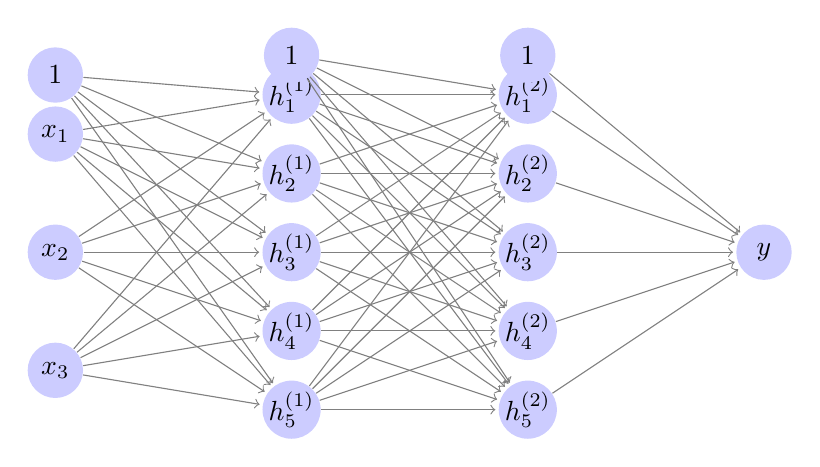
\begin{tikzpicture}[shorten >=1pt,->,draw=black!50, node distance=1.5cm]
      \tikzstyle{every neuron}=[circle,fill=blue!20,minimum size=20pt,inner sep=0pt]
      
      % Input Layer (3 neurons) + Bias node
      \node[every neuron] (I-1) at (0,-1.5) {$x_1$};
      \node[every neuron] (I-2) at (0,-3) {$x_2$};
      \node[every neuron] (I-3) at (0,-4.5) {$x_3$};
      \node[every neuron] (I-b) at (0,-0.75) {1};
      
      % First Hidden Layer (5 neurons) + Bias node
      \foreach \i in {1,...,5}
        \node[every neuron] (H1-\i) at (3,-\i*1) {$h^{(1)}_\i$};
      \node[every neuron] (H1-b) at (3,-0.5) {1};
      
      % Second Hidden Layer (5 neurons) + Bias node
      \foreach \i in {1,...,5}
        \node[every neuron] (H2-\i) at (6,-\i*1) {$h^{(2)}_\i$};
      \node[every neuron] (H2-b) at (6,-0.5) {1};
      
      % Output Layer (1 neuron)
      \node[every neuron] (O) at (9,-3) {$y$};
      
      % Connections: Input to First Hidden
      \foreach \i in {1,...,3}
        \foreach \j in {1,...,5}
          \draw (I-\i) -- (H1-\j);
      \foreach \j in {1,...,5}
          \draw (I-b) -- (H1-\j);
      
      % Connections: First Hidden to Second Hidden
      \foreach \i in {1,...,5}
        \foreach \j in {1,...,5}
          \draw (H1-\i) -- (H2-\j);
      \foreach \j in {1,...,5}
          \draw (H1-b) -- (H2-\j);
      
      % Connections: Second Hidden to Output
      \foreach \i in {1,...,5}
        \draw (H2-\i) -- (O);
      \draw (H2-b) -- (O);
    \end{tikzpicture}
    \end{center}
\end{enumerate}

\newpage

% \section{Programming Practice and Data Operation}

\end{document}
